\documentclass{article}

\author{Pedro Henrique Limeira da Cruz}
\title{ES704 - Instrumentação Básica}

\usepackage[margin=0.8in]{geometry}
\usepackage{indentfirst}
\usepackage{fancyhdr}
\usepackage{tcolorbox}
\usepackage{graphicx}
\usepackage{amsmath}
\usepackage{amssymb}
\usepackage{hyperref}

% Create a new command to be used in the align environment in multiple line equations do only the last equation is numbered  
\newcommand{\n}{\nonumber \\ }
\makeatletter
\let\inserttitle\@title
\makeatother
% Set the style of the page 
\pagestyle{fancy}
\fancyhf{}
\rhead{Pedro Henrique L. da Cruz}
\lhead{\inserttitle}
\rfoot{Page \thepage}

\hypersetup{
    colorlinks=true,
    linkcolor=black,
    filecolor=magenta,
    urlcolor=cyan,
}

% Begin the Document 
\begin{document}

    \maketitle
    \thispagestyle{empty}

    % Add the image inside a figure in as the first page
    \begin{figure}[h]
        \begin{center}
            
\includegraphics[scale = 0.15]{/Users/pedrocruz/Documents/UNICAMP/ES101/ES101 - Robotic Arm/img/unicamp.png}
        \end{center}
    \end{figure}

    % Change to the Next page 
    \newpage
    \tableofcontents
    \newpage

    \section{Medição}
        
        \subsection{Introdução}
            A principal importância de medições para sistemas mecatrônicos é de regularizar a resposta da planta de forma autônoma e contínua, fazendo com que a saída real seja igual a desejada (chamada
            de \emph{setpoint}), como mostrado no diagrama de blocos abaixo.

            \begin{figure}[h]
                \centering
                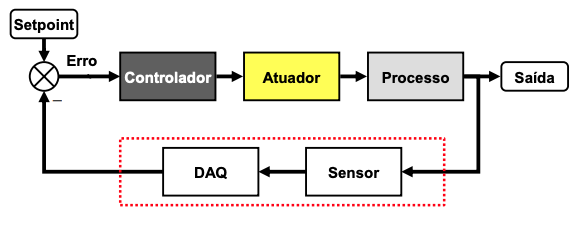
\includegraphics[width=.5\textwidth]{imgs/diag_blocos.png}
                \caption{Exemplo de uma plata/processo, representado em diagrama de blocos}
            \end{figure}

            Antes de prosseguir, entretanto, é importante definir mais cuidadosamente alguns conceitos:
            \begin{itemize}
                \item \textbf{Medição}: Atribuir valor ou tendência à variável de interesse;
                \item \textbf{Variável}: Quantidade física a ser determinada, que pode ser divida em:
                    \subitem \textbf{Dependente/Independente}: Se depende ou não de outras variáveis;
                    \subitem \textbf{Contínua/Discreta}
                    \subitem \textbf{Controlada}: O valor pode ser mantido durante o experimento;
                    \subitem \textbf{Externa}: Variável não-controlada, gera ruído e interferência;
                \item \textbf{Parâmetro}: Grupo funcional de variáveis.
            \end{itemize}

        \subsection{Sistemas de Medição}
            Aprofundando mais nos sistemas de medição, temos a seguinte planta, que representa os diferente estágios necessários para uma medição por sensores:

            \begin{figure}[h]
                \centering
                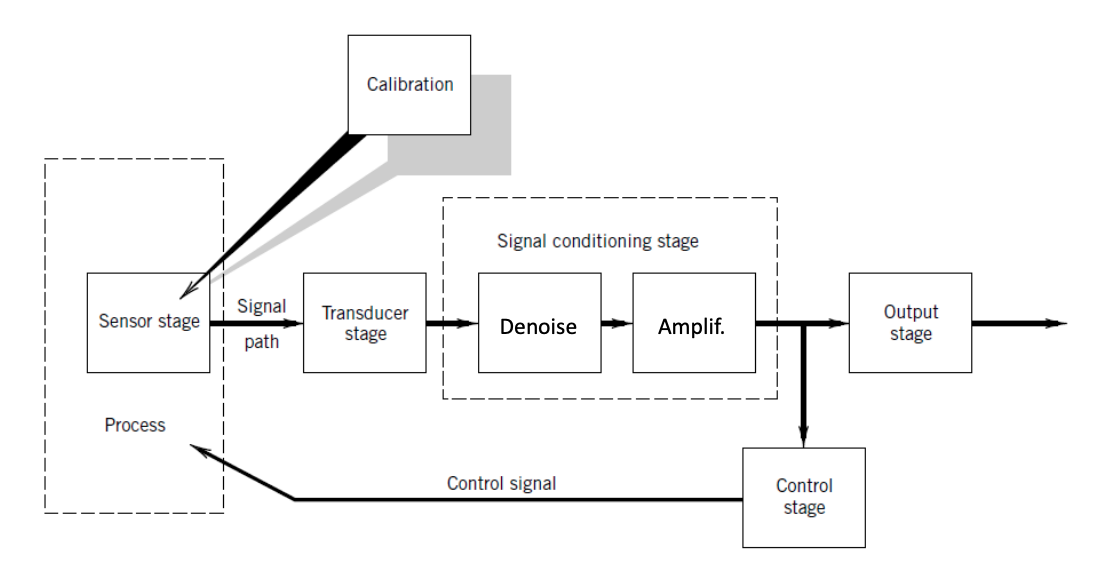
\includegraphics[width=.7\textwidth]{imgs/sys_medi.png}
                \caption{Sistema Geral de Medição - Diagrama de Blocos}
            \end{figure}

            A planta de medição possui:
            \begin{itemize}
                \item \textbf{Sinais}: Valores Transmitidos entre os estágios do sistema;
                \item \textbf{Sensor}: Converte o fenômeno físico em uma variável medida - Detecta mudança de quantidades físicas;
                \item \textbf{Transdutor}: Converte o sinal do sensor em uma saída mensurável (elétrica, mec, ...) - Transforma uma forma de Energia em Outra;
                \item \textbf{Condicionamento de Sinais}: Amplificação, Filtragem, ...
                \item \textbf{Saída}: Indica ou armazena a variável medida;
                \item \textbf{Controle}: Retifica o sistema para minimizar o erro de medição.
            \end{itemize}

        \subsection{Calibração}
            Podemos verificar no diagrama anterior que há a necessidade da calibração do sensor, \emph{i.e}, determinar matematicamente a relação entrada-saída do sistema.
            Para tal, é necessário aplicar excitações de entrada conhecidas, aferidas com um \textbf{padrão} ou instrumento de referência, e medirmos a saída, para podermos gerar um modelo matemático,
            relacionando entrada-saída.

            A calibração pode ser:
            \begin{itemize}
                \item Estática
                \item Dinâmica
            \end{itemize}

            \subsubsection{Calibração Estática}
                \begin{figure}[h]
                    \centering
                    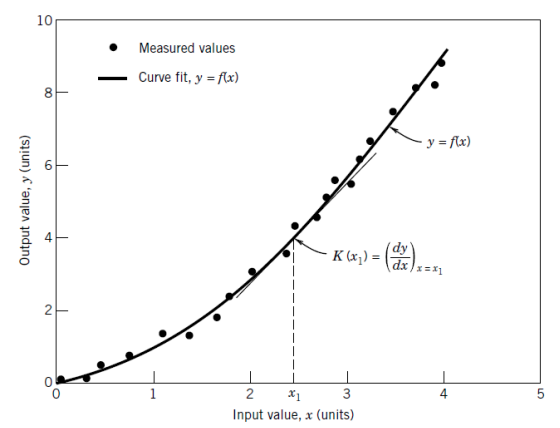
\includegraphics[width=.5\textwidth]{imgs/curve_fitting_est.png}
                    \caption{Exemplo de Curve Fit}
                \end{figure}

                A calibração estática é a mais simples, pois se aplica uma entrada conhecida, espera-se o sistema convergir (a extinção da parte transiente do sinal) e então mede a sua resposta.
                Ao final, teremos uma série de pontos e função de entradas definidas ($y = f(x)$), e ao final podemos usar diferentes métodos de \emph{curve-fitting} para modelarmos o comportamento do
                sistema (como exemplificado pela imagem acima), ou ainda interpolar para valores de entradas novos.

                Uma medida extremamente importante para a calibração estática é a \emph{sensibilidade estática}, também chamada de \emph{ganho}, que caracteriza a relação de amplitude entre a entrada
                e a saída, dada por:
                \begin{align}
                    K = \frac{df(x)}{dx} \bigg\rvert_{x=x_0} \label{eq:ganho_calib_estatica}
                \end{align}

                Além disso, definimos também o \emph{range} do sensor como sendo o intervalo no qual a curva de calibração é válida. Fora deste intervalo a resposta é \textbf{extrapolada}.
                \begin{align}
                    r_i = x_{max}-x_{min} \\
                    r_o = y_{max}-y_{min}
                \end{align}

                Por fim, temos ainda que definir a \textbf{resolução} do sensor, \emph{i.e} o menor incremento que pode ser detectado pelo sistema de medição e definir o \textbf{Limiear} (também
                chamado de \textbf{Threshold}) do sensor, que é o valor mínimo de estimulo necessário para que o sistema gere incremento em sua resposta.

            \subsubsection{Calibração Dinâmica}




    
\end{document}